\documentclass{article}

%%\VignetteIndexEntry{A Lego System for Conditional Inference}
%%\VignetteDepends{coin}

\usepackage{amstext}
\usepackage{amsfonts}
\usepackage{hyperref}
\usepackage[round]{natbib}
\renewcommand{\refname}{REFERENCES}
\usepackage{hyperref}
\usepackage{graphicx}
\usepackage{rotating}
%%\usepackage[nolists]{endfloat}

\newcommand{\Rpackage}[1]{\textit{#1}}
\newcommand{\Robject}[1]{\texttt{#1}}
\newcommand{\Rclass}[1]{\textit{#1}}
\newcommand{\Rcmd}[1]{\texttt{#1}}
\newcommand{\Roperator}[1]{\texttt{#1}}
\newcommand{\Rarg}[1]{\texttt{#1}}
\newcommand{\Rlevel}[1]{\texttt{#1}}

\newcommand{\RR}{\textsf{R}} 
\renewcommand{\S}{\textsf{S}}

\newcommand{\R}{\mathbb{R} }
\newcommand{\Prob}{\mathbb{P} }
\newcommand{\N}{\mathbb{N} }
\newcommand{\C}{\mathbb{C} }
\newcommand{\V}{\mathbb{V}} %% cal{\mbox{\textnormal{Var}}} }
\newcommand{\E}{\mathbb{E}} %%mathcal{\mbox{\textnormal{E}}} }
\newcommand{\Var}{\mathbb{V}} %%mathcal{\mbox{\textnormal{Var}}} }
\newcommand{\argmin}{\operatorname{argmin}\displaylimits}
\newcommand{\argmax}{\operatorname{argmax}\displaylimits}
\newcommand{\LS}{\mathcal{L}_n}
\newcommand{\TS}{\mathcal{T}_n}
\newcommand{\LSc}{\mathcal{L}_{\text{comb},n}}
\newcommand{\LSbc}{\mathcal{L}^*_{\text{comb},n}}
\newcommand{\F}{\mathcal{F}}
\newcommand{\A}{\mathcal{A}}
\newcommand{\yn}{y_{\text{new}}}
\newcommand{\z}{\mathbf{z}}
\newcommand{\X}{\mathbf{X}}
\newcommand{\Y}{\mathbf{Y}}
\newcommand{\sX}{\mathcal{X}}
\newcommand{\sY}{\mathcal{Y}}
\newcommand{\T}{\mathbf{T}}
\newcommand{\x}{\mathbf{x}}
\renewcommand{\a}{\mathbf{a}}
\newcommand{\xn}{\mathbf{x}_{\text{new}}}
\newcommand{\y}{\mathbf{y}}
\newcommand{\w}{\mathbf{w}}
\newcommand{\ws}{\mathbf{w}_\cdot}
\renewcommand{\t}{\mathbf{t}}
\newcommand{\M}{\mathbf{M}}
\renewcommand{\vec}{\text{vec}}
\newcommand{\B}{\mathbf{B}}
\newcommand{\K}{\mathbf{K}}
\newcommand{\W}{\mathbf{W}}
\newcommand{\D}{\mathbf{D}}
\newcommand{\I}{\mathbf{I}}
\newcommand{\bS}{\mathbf{S}}
\newcommand{\cellx}{\pi_n[\x]}
\newcommand{\partn}{\pi_n(\mathcal{L}_n)}
\newcommand{\err}{\text{Err}}
\newcommand{\ea}{\widehat{\text{Err}}^{(a)}}
\newcommand{\ecv}{\widehat{\text{Err}}^{(cv1)}}
\newcommand{\ecvten}{\widehat{\text{Err}}^{(cv10)}}
\newcommand{\eone}{\widehat{\text{Err}}^{(1)}}
\newcommand{\eplus}{\widehat{\text{Err}}^{(.632+)}}
\newcommand{\eoob}{\widehat{\text{Err}}^{(oob)}}

\RequirePackage[T1]{fontenc}
\RequirePackage{graphicx,ae,fancyvrb}
\IfFileExists{upquote.sty}{\RequirePackage{upquote}}{}
\usepackage{relsize}

\DefineVerbatimEnvironment{Sinput}{Verbatim}{baselinestretch=1}
\DefineVerbatimEnvironment{Soutput}{Verbatim}{fontfamily=courier,
                                              baselinestretch=1,
                                              fontshape=it,
                                              fontsize=\relsize{-1}}
\DefineVerbatimEnvironment{Scode}{Verbatim}{}
\newenvironment{Schunk}{}{}

\renewcommand{\baselinestretch}{1}



\hypersetup{%
  pdftitle = {A Lego System for Conditional Inference},
  pdfsubject = {Manuscript},
  pdfauthor = {Torsten Hothorn, Kurt Hornik,
               Mark A. van de Wiel and Achim Zeileis},
%% change colorlinks to false for pretty printing
  colorlinks = {true},
  linkcolor = {blue},
  citecolor = {blue},
  urlcolor = {red},
  hyperindex = {true},
  linktocpage = {true},
}



\begin{document}

\title{A Lego System for Conditional Inference}

\author{Torsten Hothorn$^1$, Kurt Hornik$^2$, \\ 
            Mark A. van de Wiel$^3$ and Achim Zeileis$^2$}
\setkeys{Gin}{width=0.9\textwidth}

\date{}

\maketitle

\thispagestyle{empty}

\noindent$^1$ Institut f\"ur Medizininformatik, Biometrie und Epidemiologie\\
           Friedrich-Alexander-Universit\"at Erlangen-N\"urnberg\\
           Waldstra{\ss}e 6, D-91054 Erlangen, Germany \\
           \texttt{Torsten.Hothorn@R-project.org}
         \newline

         \noindent$^2$ Department f\"ur Statistik und Mathematik,
            Wirtschaftsuniversit\"at Wien \\
            Augasse 2-6, A-1090 Wien, Austria \\
            \texttt{Kurt.Hornik@R-project.org} \\
            	exttt{Achim.Zeileis@R-project.org}
         \newline

         \noindent$^3$ Department of Mathematics and Computer Science \\
            Eindhoven University of Technology \\
            HG 9.25, P.O. Box 513 \\
            5600 MB Eindhoven, The Netherlands \\
            \texttt{m.a.v.d.wiel@TUE.nl}
         \newline

\begin{abstract}
Conditioning on the observed data is an important and flexible 
design principle for statistical test procedures. Although generally
applicable, permutation tests currently in use are limited to 
the treatment of special cases, such as contingency tables or $K$-sample
problems. A new theoretical framework for permutation
tests opens up the way to a unified and generalized view. We argue that the
transfer of such a theory to practical data analysis has important
implications in many applications and requires tools that enable the
data analyst to compute on the theoretical concepts as closely as possible.
We re-analyze four data sets
by adapting the general conceptual framework to these non-standard inference procedures
and
utilizing the \Rpackage{coin} add-on package in the \RR{} system for statistical computing
to show what one can gain from going beyond the `classical' test procedures.
\end{abstract}

\noindent
KEY WORDS: Permutation tests; Multiple testing; Independence; Software.
\newline

\newpage

\section{INTRODUCTION}

The distribution of a test statistic under the circumstances of a certain
null hypothesis clearly depends on the unknown distribution of the data and
thus is unknown as well.
Two concepts are commonly applied to dispose of this dependency.
Unconditional tests impose assumptions on the distribution of the data such
that the null distribution of a test statistic can be derived analytically. In contrast, 
conditional tests
replace the unknown null distribution by the conditional null distribution,
i.e., the distribution of the test statistic given the observed data. The
latter approach is known as \textit{permutation testing} and was developed
by R. A. Fisher more than 70 years ago \citep{Fisher1935}. 
The pros and cons of both approaches in different fields of application 
have been widely discussed \citep[e.g.~by][]{why-permut:1998,pros-and-c:2000,Shuster2005}.
Here, we focus on the practical aspects of permutation testing rather than
dealing with its methodological foundations.

For the construction of permutation tests it is common exercise to `recycle'
test statistics well known from the unconditional world, such as linear rank
statistics, ANOVA $F$ statistics or $\chi^2$ statistics for
contingency tables, and to replace the unconditional null distribution with
the conditional distribution of the test statistic under the null
hypothesis \citep{Edgington1987,Good2000,Pesarin2001,Ernst2004}. 
Because the choice of the test statistic is the only `degree of freedom' for
the data analyst,
the classical view on permutation tests requires 
a `cook book' classification of inference problems (categorical data
analysis, multivariate analysis, $K$-sample location problems, correlation,
etc.), each being associated with a `natural' form of the test statistic.

The theoretical advances of the last decade \citep[notably][]{StrasserWeber1999,JanssenPauls2003}
give us a much better understanding of the strong connections between the 
`classical' permutation tests defined for different inference problems. 
As we will argue in this paper, the new
theoretical tools open up the way to a simple construction principle 
for test procedures in new and challenging inference problems.
Especially attractive for this purpose is the theoretical framework for
permutation tests developed by \cite{StrasserWeber1999}. This unifying
theory is based on a flexible form of multivariate linear statistics for the
general independence problem. 

This framework provides us with a conceptual Lego system for the construction
of permutation tests consisting of Lego bricks for linear statistics
suitable for different inference problems (contingency tables, multivariate
problems, etc.), different forms of test statistics, such as quadratic forms
for global tests or test statistics suitable for multiple comparison
procedures, and several ways to compute or approximate the conditional null
distribution. The classical procedures, such as a permutation $t$ test, are part
of this framework and, even more interestingly, new test procedures can be
embedded into the same theory whose main ideas are sketched in
Section~\ref{CI}.

Currently, the statistician's toolbox consists of rather inflexible spanners,
such as the Wilcoxon-Mann-Whitney test for comparing two distributions 
or the Cochran-Mantel-Haenszel $\chi^2$ test for independence in
contingency tables. With this work, we add an adjustable spanner to the 
statistician's toolbox which helps to address both the common as well 
as new or unusual inference problems with the appropriate 
conditional test procedures. In the main part of this paper we show how one can
construct and implement permutation tests `on the fly' by plugging together Lego bricks for
the multivariate linear statistic, the test statistic and the conditional
null distribution, both conceptually and practically by means of the 
\Rpackage{coin} add-on package 
 \citep{PKG:coin} in the \RR{} system for statistical computing
\citep{Rcore2005}.


\section{A CONCEPTUAL LEGO SYSTEM \label{CI}}

To fix notations,
we assume that we are provided with observations
$(\Y_i, \X_i)$ for $i = 1, \dots, n$.
The variables $\Y$ and $\X$ from sample spaces $\mathcal{Y}$ and
$\mathcal{X}$ may
be measured at arbitrary scales and may be multivariate as well. 
We are interested in testing the null hypothesis of independence of $\Y$ and $\X$
\begin{eqnarray*}
H_0: D(\Y | \X) = D(\Y)
\end{eqnarray*}
against arbitrary alternatives. \cite{StrasserWeber1999} suggest to derive
\textit{scalar} test statistics for testing $H_0$ from \textit{multivariate}
linear statistics of the form 
\begin{eqnarray*}
\T = \vec\left(\sum_{i = 1}^n g(\X_i) h(\Y_i)^\top\right)
\in \R^{pq \times 1}.
\end{eqnarray*}
Here, $g: \mathcal{X} \rightarrow \R^{p \times 1}$ is a transformation of
the $\X$ measurements and $h: \mathcal{Y} \rightarrow
\R^{q \times 1}$ is called \emph{influence function}. The function $h(\Y_i)
= h(\Y_i, (\Y_1, \dots, \Y_n))$ must depend on the responses $(\Y_1, \dots, \Y_n)$ in a permutation
symmetric way. We will give several examples how to choose $g$ and $h$
for specific inference problems in Section~\ref{play}.

The distribution of $\T$  depends on the joint distribution of $\Y$ and $\X$, 
which is unknown under almost all practical circumstances. 
At least under the null hypothesis one can dispose of this 
dependency by fixing $\X_1, \dots, \X_n$ and conditioning on all possible 
permutations $S$ of the responses $\Y_1, \dots, \Y_n$. 

The conditional expectation $\mu \in \R^{pq \times 1}$ and covariance
$\Sigma \in \R^{pq \times pq}$ of $\T$ under $H_0$ given
all permutations $\sigma \in S$ of the responses are derived by
\cite{StrasserWeber1999}:
\begin{eqnarray*}
\mu = \E(\T | S) & = & \vec \left( \left( \sum_{i = 1}^n g(\X_i) \right)
\E(h | S)^\top \right) \\
\Sigma = \V(\T | S) & = &
    \frac{n}{n - 1}  \V(h | S) \otimes
        \left(\sum_i g(\X_i) \otimes  g(\X_i)^\top \right)
\\
& - & \frac{1}{n - 1}  \V(h | S)  \otimes \left(
        \sum_i g(\X_i) \right) \otimes \left( \sum_i g(\X_i)\right)^\top
\nonumber
\end{eqnarray*}
where $\otimes$ denotes the Kronecker product, and the conditional
expectation of the influence function is $\E(h | S) = n^{-1} \sum_i
h(\Y_i)$ with corresponding $q \times q$ covariance matrix
\begin{eqnarray*}
\V(h | S) = n^{-1} \sum_i \left(h(\Y_i) - \E(h | S) \right) \left(h(\Y_i) - \E(h | S)\right)^\top.
\end{eqnarray*}

The key step for the construction of test statistics based on the multivariate
linear statistic $\T$ is its standardization utilizing the 
conditional expectation $\mu$ and covariance matrix $\Sigma$. 
Univariate test statistics~$c$ mapping a linear
statistic $\T \in \R^{pq \times 1}$ 
into the real line can be of arbitrary form.  An obvious choice is
the maximum of the absolute values of the standardized linear statistic
\begin{eqnarray*}
c_\text{max}(\T, \mu, \Sigma)  = \max \left| \frac{\T -
\mu}{\text{diag}(\Sigma)^{1/2}} \right|.
\end{eqnarray*}
A prominent alternative are quadratic forms 
$c_\text{quad}(\T, \mu, \Sigma)  =
(\T - \mu) \Sigma^+ (\T - \mu)^\top$ involving 
the Moore-Penrose inverse $\Sigma^+$ of $\Sigma$.

%%The definition of one- and two-sided $p$-values used for the computations in
%%the \Rpackage{coin} package is
%%\begin{eqnarray*}
%%& & P(c(\T, \mu, \Sigma)\le c(\mathbf{t}, \mu, \Sigma)) \quad \text{(less)} \\  
%%& & P(c(\T, \mu, \Sigma) \ge c(\mathbf{t}, \mu, \Sigma)) \quad \text{(greater)}\\
%%& & P(|c(\T, \mu, \Sigma)| \le |c(\mathbf{t}, \mu, \Sigma)|) \quad
%%\text{(two-sided).}
%%\end{eqnarray*}
%%Note that for quadratic forms only two-sided $p$-values are available 
%%and that in the one-sided case maximum type test statistics are replaced by
%%\begin{eqnarray*}
%%\min \left( \frac{\mathbf{t} - \mu}{\text{diag}(\Sigma)^{1/2}} \right)
%%    \quad \text{(less) and } 
%%\max \left( \frac{\mathbf{t} - \mu}{\text{diag}(\Sigma)^{1/2}} \right)
%%    \quad \text{(greater).}
%%\end{eqnarray*}

The conditional distribution $\Prob(c(\T, \mu, \Sigma) \le z | S)$
is the number of permutations $\sigma \in S$ of the data 
with corresponding test statistic not exceeding $z$ divided by the total number
of permutations in $S$. For some special forms of the
multivariate linear statistic the exact distribution of some 
test statistics is trackable for small and moderate sample sizes.
%%For two-sample problems, the shift-algorithm by \cite{axact-dist:1986} 
%%and \cite{exakte-ver:1987} and the split-up algorithm by 
%%\cite{vdWiel2001} are implemented as part of the package.
Conditional Monte-Carlo procedures (`resampling') can always be used to 
approximate the exact distribution up to any desired accuracy by evaluating
the test statistic for a random sample from the set of all permutations $S$.
It is important to note that in the presence of a grouping of the observations
into blocks, only permutations within blocks are eligible and that the
conditional expectation and covariance matrix need to be computed
separately for each block.

Less well known is the fact that 
the conditional distribution can be approximated by its limiting distribution
under all circumstances. \cite{StrasserWeber1999} showed in their Theorem~2.3 that the   
conditional distribution of linear statistics $\T$ with conditional    
expectation $\mu$ and covariance $\Sigma$ tends to a multivariate normal
distribution with parameters $\mu$ and $\Sigma$ as $n \rightarrow
\infty$. Thus, the asymptotic conditional distribution of test statistics of
the form $c_\text{max}$ is normal and
can be computed directly in the univariate case ($pq = 1$) and by numerical 
algorithms in the multivariate case \citep[e.g., using the quasi-randomized
Monte-Carlo procedures of][]{numerical-:1992}.
For quadratic forms
$c_\text{quad}$ which follow a $\chi^2$ distribution with degrees of freedom
given by the rank of $\Sigma$ \citep[e.g.~Theorem 6.20, ][]{Rasch1995}, exact
probabilities can be computed efficiently.

\section{PLAYING LEGO \label{play}}

The Lego system sketched in the previous section consists of Lego bricks for 
the multivariate linear statistic $\T$, namely the transformation $g$ and
influence function $h$, multiple forms of the test statistic $c$ and several choices
of approximations of the null distribution. In this section, we will show how
classical procedures, starting with the conditional Kruskal-Wallis test and
the Cochran-Mantel-Haenszel test, can be embedded into this general theory
and, much more interesting from our point of view, how new conditional test
procedures can be constructed conceptually \textit{and} practically. 
Therefore, each inference problem comes with \RR{} code performing the
appropriate conditional test using the \Rpackage{coin} functionality 
which enables the data analyst to benefit from this
simple methodology in every day's data analysis. All analyses are
reproducible from the \Rpackage{coin} package vignette available from
\url{http://CRAN.R-project.org/}.

\paragraph{Genetic Components of Alcoholism.}

Various studies have linked alcohol dependence phenotypes to chromosome 4.  
One candidate gene is \textit{NACP} (non-amyloid component of plaques), 
coding for alpha synuclein. 
\cite{Boenscheta2005} found longer alleles of
\textit{NACP}-REP1 in alcohol-dependent patients compared with healthy controls
and report that the allele lengths show some
association with levels of expressed alpha synuclein mRNA (see
Figure~\ref{alpha-box}).

\setkeys{Gin}{width=0.7\textwidth}

\begin{figure}
\begin{center}
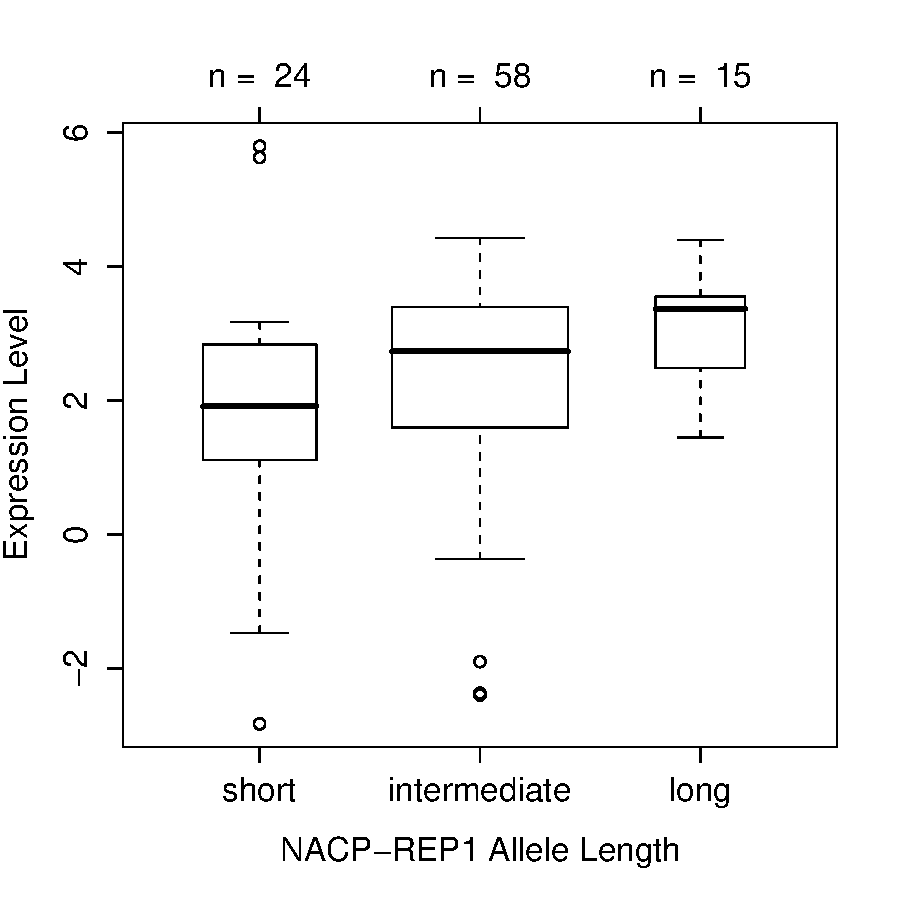
\includegraphics{LegoCondInf-alpha-data-figure}
\caption{\Robject{alpha} data: Distribution of levels of expressed alpha synuclein mRNA
         in three groups defined by the \textit{NACP}-REP1 allele lengths.
         \label{alpha-box}}
\end{center}
\end{figure}

\setkeys{Gin}{width=\textwidth}

Our first attempt to test for different levels of gene expression in the three
groups is the classical Kruskal-Wallis test. Here, the transformation 
$g$ is a dummy coding of the allele length ($g(\X_i) = (0, 1, 0)^\top$ for
intermediate length, for example) and the value of the influence function 
$h(\Y_i)$ is the rank of $\Y_i$ among the ranks of $\Y_1, \dots, \Y_n$.
Thus, the linear statistic $\T$ is the vector of rank sums in each of the 
three groups and the test statistic is a quadratic form 
$(\T - \mu) \Sigma^+ (\T - \mu)^\top$ 
utilzing the conditional expectation~$\mu$ and covariance matrix~$\Sigma$.

In order to compute the linear statistic we need to define an
influence function performing a ranking of the expression levels.
Under the null hypothesis, the $c_\text{quad}$-type Kruskal-Wallis 
test statistic tends to a $\chi^2$
distribution with two degrees of freedom (the rank of the conditional
covariance matrix $\Sigma$) from which a $p$-value can be
computed. In \RR{}, the function \Rcmd{independence\_test} takes a formula
describing the inference problem, i.e., the independence of expression
levels (\Robject{elevel}) and allele lengths (\Robject{alength}), the
influence function is specified via the \Rcmd{ytrafo} argument and we ask
for a $c_\text{quad}$-type test statistic (\Rcmd{teststat}) as follows:
\begin{Schunk}
\begin{Sinput}
R> independence_test(elevel ~ alength, data = alpha, 
+     ytrafo = function(data) trafo(data, numeric_trafo = rank), 
+     teststat = "quad")
\end{Sinput}
\begin{Soutput}
	Asymptotic General Independence Test

data:  elevel by groups short, intermediate, long 
T = 8.8302, df = 2, p-value = 0.01209
\end{Soutput}
\end{Schunk}
The results are equivalent to the results reported by \Rcmd{kruskal.test},
the `classical' interface to the Kruskal-Wallis test in \RR{}
\begin{Schunk}
\begin{Sinput}
R> kruskal.test(elevel ~ alength, data = alpha)
\end{Sinput}
\begin{Soutput}
	Kruskal-Wallis rank sum test

data:  elevel by alength 
Kruskal-Wallis chi-squared = 8.8302, df = 2, p-value =
0.01209
\end{Soutput}
\end{Schunk}
However, going beyond the functionality implemented in \Rcmd{kruskal.test}
would require extensive programming but is easily possible with the
\Rpackage{coin} functionality being available. For example, 
ignoring the ordinal structure of the allele length is only
suboptimal, especially when we have an ordered alternative in mind. 
Ordinal variables can be incorporated into the general framework
via linear-by-linear association tests \citep{Agresti2002}. 
When $\X$ is measured at $K$ levels associated with a score vector 
$\gamma \in \R^{K \times 1}$, the linear statistic reads
\begin{eqnarray*}
\T_\gamma = \vec \left( \sum_{i=1}^n \gamma^\top g(\X_i)
            h(\Y_i)^\top \right).
\end{eqnarray*}
Here, the mid-points of the intervals used to categorize the allele lengths
are a possible choice for the score vector $\gamma$ and the linear-by-linear
association test can be performed by attaching the scores to the variable
\Robject{alength}:
\begin{Schunk}
\begin{Sinput}
R> independence_test(elevel ~ alength, data = alpha, 
+     ytrafo = function(data) trafo(data, numeric_trafo = rank), 
+     scores = list(alength = c(2, 7, 11)))
\end{Sinput}
\begin{Soutput}
	Asymptotic General Independence Test

data:  elevel by
	 groups short < intermediate < long 
T = 2.9263, p-value = 0.003430
alternative hypothesis: two.sided 
\end{Soutput}
\end{Schunk}
The smaller $p$-value corresponds well with Figure~\ref{alpha-box}, i.e., 
the impression that the expression levels increase with increasing 
allele lengths. 

\paragraph{Smoking and Alzheimer's Disease.}


\cite{SalibHillier1997} report results of a case-control study on
Alzheimer's disease and smoking behavior of 
$198$
patients suffering from Alzheimer's disease and 
$164$
controls. The data shown in Table~\ref{alzheimertab} have been 
re-constructed from Table~4 in \cite{SalibHillier1997} and are depicted in
Figure~\ref{alz-plot}. 
The authors conclude that `cigarette smoking is less frequent in 
men with Alzheimer's disease.' 

\begin{table}[h]
\begin{center}
\caption{\Robject{alzheimer} data: Smoking and Alzheimer's disease. \label{alzheimertab}}
\begin{tabular}{lrrrr} \hline \hline
 & \multicolumn{4}{c}{No. of cigarettes daily} \\
 & None & <10 & 10--20 & >20 \\ \hline
\textit{Female} & & & & \\
Alzheimer's  &  91 & 7 & 15 & 21 \\ 
Other dementias  &  55 & 7 & 16 & 9 \\ 
Other diagnoses  &  80 & 3 & 25 & 9 \\ 
& & & & \\
\textit{Male} & & & & \\
Alzheimer's  &  35 & 8 & 15 & 6 \\ 
Other dementias  &  24 & 1 & 17 & 35 \\ 
Other diagnoses  &  24 & 2 & 22 & 11 \\ \hline
\end{tabular}
\end{center}
\end{table}

\begin{figure}
\begin{center}
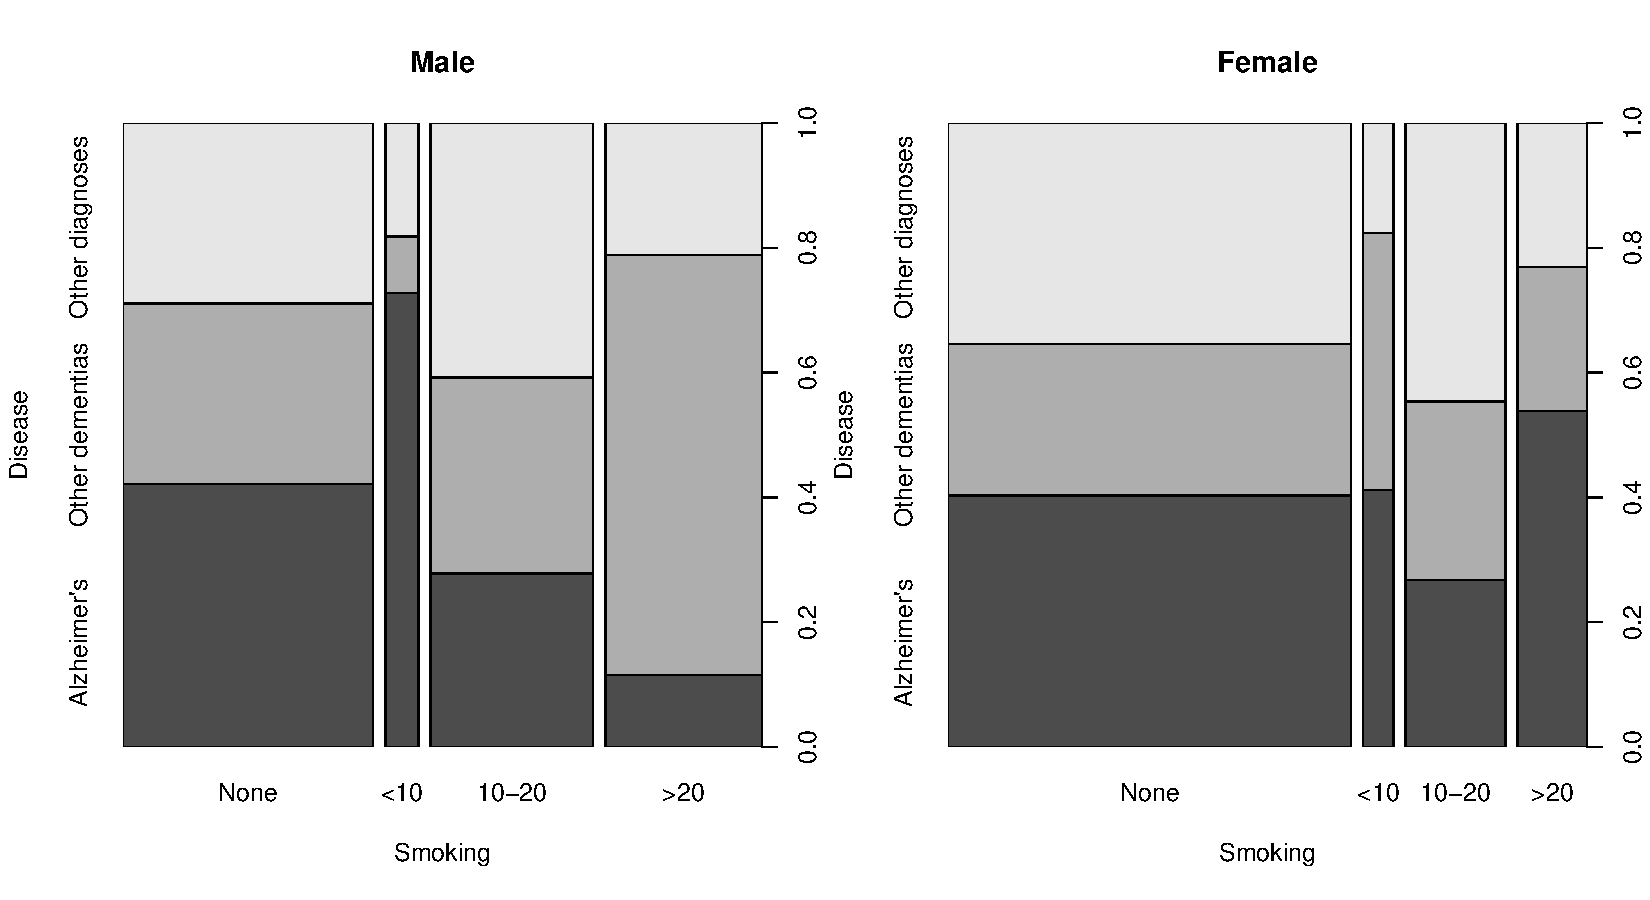
\includegraphics{LegoCondInf-alzheimer-plot}
\caption{\Robject{alzheimer} data: Association of
smoking behavior and disease status stratified by gender. \label{alz-plot}}
\end{center}
\end{figure}

We are interested to assess whether there is any association
between smoking and Alzheimer's (or other dementia) diseases and, in a
second step, how a potential association can be described. First,
the global null hypothesis of independence between smoking behavior and disease
status for both females and males, i.e., treating gender as a
block factor, can be tested with a $c_\text{quad}$-type test statistic, i.e., the 
Cochran-Mantel-Haenszel test:
\begin{Schunk}
\begin{Sinput}
R> it_alz <- independence_test(disease ~ smoking | gender, 
+     data = alzheimer, teststat = "quad")
R> it_alz
\end{Sinput}
\begin{Soutput}
	Asymptotic General Independence Test

data:  disease by
	 groups None, <10, 10-20, >20 
	 stratified by gender 
T = 23.3163, df = 6, p-value = 0.0006972
\end{Soutput}
\end{Schunk}
which suggests that there is a clear deviation from independence. 
By default, the influence function $h$ and the transformation $g$ 
are dummy codings of the disease status $\Y$ and the smoking behavior $\X$, 
i.e., $h(\Y_i) = (1, 0, 0)^\top$ 
and $g(\X_i) = (1, 0, 0 ,0)^\top$ for a non-smoking Alzheimer patient. 
Consequently, the linear multivariate statistic $\T$ based on $g$ and $h$ 
is the contingency table of both variables 
\begin{Schunk}
\begin{Sinput}
R> statistic(it_alz, type = "linear")
\end{Sinput}
\begin{Soutput}
      Alzheimer's Other dementias Other diagnoses
None          126              79             104
<10            15               8               5
10-20          30              33              47
>20            27              44              20
\end{Soutput}
\end{Schunk}
with conditional expectation \Rcmd{expectation(it\_alz)} and conditional
covariance \Rcmd{covariance(it\_alz)} which are available for standardizing
the contingency table $\T$. The conditional distribution is approximated by
its limiting $\chi^2$ distribution by default. 

Given that there is significant departure from independence, we further
investigate the structure of association between smoking and Alzheimer's
disease. First we assess for which gender the violation of independence 
occured
\begin{Schunk}
\begin{Sinput}
R> females <- alzheimer$gender == "Female"
R> pvalue(independence_test(disease ~ smoking, data = alzheimer, 
+     subset = females, teststat = "quad"))
\end{Sinput}
\begin{Soutput}
[1] 0.09060652
\end{Soutput}
\begin{Sinput}
R> pvalue(independence_test(disease ~ smoking, data = alzheimer, 
+     subset = !females, teststat = "quad"))
\end{Sinput}
\begin{Soutput}
[1] 3.169418e-06
\end{Soutput}
\end{Schunk}
where it turns out that the association is due to the male patients only
(see also Figure~\ref{alz-plot}). Thus, we focus on the male patients in 
the following.
Furthermore, a $c_\text{quad}$-type test statistic is not particularly useful 
for gaining insight into the association structure of contingency tables
because the contributions of all cells are collapsed in such a quadratic form.
Instead, we define the test statistic as the maximum of the 
standardized contingency table via
\begin{Schunk}
\begin{Sinput}
R> it_alzmax <- independence_test(disease ~ smoking, 
+     data = alzheimer, subset = !females, teststat = "max")
R> it_alzmax
\end{Sinput}
\begin{Soutput}
	Asymptotic General Independence Test

data:  disease by groups None, <10, 10-20, >20 
T = 4.9504, p-value = 1.148e-05
\end{Soutput}
\end{Schunk}
where the underlying standardized contingency table highlights the cells with
deviations from independence
\begin{Schunk}
\begin{Sinput}
R> statistic(it_alzmax, "standardized")
\end{Sinput}
\begin{Soutput}
      Alzheimer's Other dementias Other diagnoses
None    2.5900465       -2.340275      -0.1522407
<10     2.9713093       -2.056864      -0.8446233
10-20  -0.7765307       -1.237441       2.1146396
>20    -3.6678046        4.950373      -1.5303056
\end{Soutput}
\end{Schunk}
This leads to the impression that heavy smokers suffer less frequently
from Alzheimer's disease but more frequently from other dementias
than expected under independence.
However, interpreting the standardized contingency table requires
knowledge about the distribution of the standardized statistics, 
e.g., via an approximation of the $95\%$ quantile of the permutation 
null distribution which is available from
\begin{Schunk}
\begin{Sinput}
R> qperm(it_alzmax, 0.95)
\end{Sinput}
\begin{Soutput}
[1] 2.813175
\end{Soutput}
\end{Schunk}
or alternatively (and more conveniently) by
switching to $p$-values adjusted for multiple testing:
\begin{Schunk}
\begin{Sinput}
R> pvalue(it_alzmax, method = "single-step")
\end{Sinput}
\begin{Soutput}
      Alzheimer's Other dementias Other diagnoses
None  0.092374157    1.707036e-01       0.9999984
<10   0.031734006    3.066296e-01       0.9719409
10-20 0.981658513    8.419042e-01       0.2751252
>20   0.002635631    2.814171e-05       0.6615635
\end{Soutput}
\end{Schunk}
These results support the conclusion that the rejection of the 
null hypothesis of independence is due to a large number of patients
with other dementias and a small number with Alzheimer's disease in the heavy
smoking group. In addition, there is some evidence that, for the small
group of men smoking less than ten cigarettes per day, the reverse
association is true.

\paragraph{Photococarcinogenicity Experiments.}

The effect on tumor frequency and latency in photococarcinogenicity
experiments, where carcinogenic doses of ultraviolet radiation (UVR) are
administered, are measured by means of (at least) three response variables:
the survival time, the time to first tumor and the total number of tumors of
animals in different treatment groups. 
The main interest is testing the global null of no treatment 
effect with respect to any of the three responses survival time, time to first tumor or
number of tumors \citep[][analyze the detection time
of tumors in addition, this data is not given here]{Molefeetal2005}. 
In case the  global null hypothesis can be rejected, the deviations 
from the partial hypotheses are of special interest.

\cite{Molefeetal2005} report data of an experiment where
$108$ animals were exposed to different levels 
of UVR exposure (group A: topical vehicle and 600 Robertson--Berger units 
of UVR, group B: no topical vehicle and 600 Robertson--Berger units of UVR and group C: 
no topical vehicle and 1200 Robertson--Berger units of UVR). 
The data are taken from Tables~1 to 3 in \cite{Molefeetal2005}, where a 
parametric test procedure is proposed. Figure
\ref{photocarfig} depicts the group effects for all three response
variables. 


\begin{figure}
\begin{center}
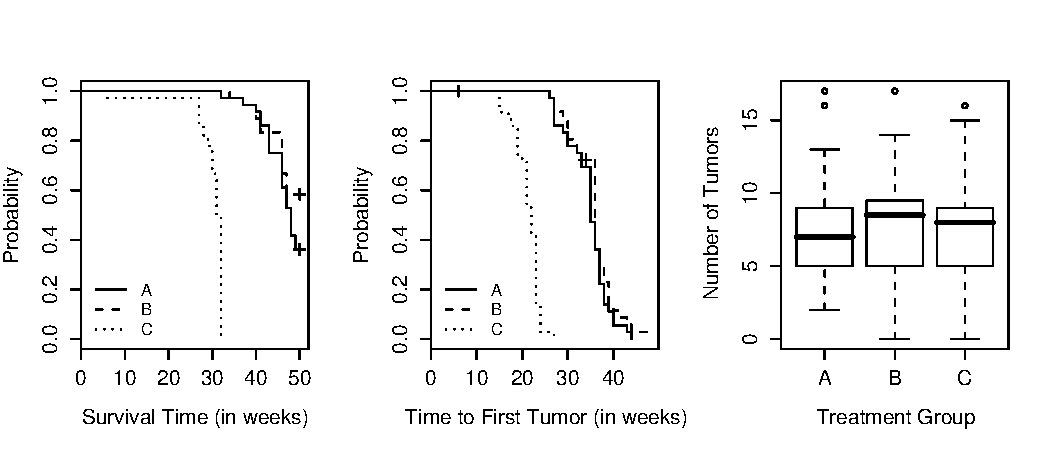
\includegraphics{LegoCondInf-photocar-plot}
\caption{\Robject{photocar} data: 
         Kaplan-Meier estimates of time to death and time to first tumor as
         well as boxplots of the total number of tumors in three treatment
         groups. \label{photocarfig}}
\end{center}
\end{figure}

First, we construct a global test for the null hypothesis of independence
of treatment and \textit{all} three response variables. A
$c_\text{max}$-type test based on the standardized multivariate          
linear statistic and an approximation of the conditional distribution
utilizing the asymptotic distribution simply reads
\begin{Schunk}
\begin{Sinput}
R> it_ph <- independence_test(Surv(time, event) + Surv(dmin, 
+     tumor) + ntumor ~ group, data = photocar)
R> it_ph
\end{Sinput}
\begin{Soutput}
	Asymptotic General Independence Test

data:  Surv(time, event), Surv(dmin, tumor), ntumor by groups A, B, C 
T = 7.0777, p-value = 7.378e-12
\end{Soutput}
\end{Schunk}
Here, the influence function $h$ consists of the logrank scores of the survival
time and time to first tumor as well as the number of tumors, i.e., for the 
first animal in the first group $h(\Y_1) =
( -1.08,-0.56,5 )^\top$
and $g(\X_1) = (1, 0, 0)^\top$. The multivariate statistic is the sum of each of
the three elements of the influence function $h$ in each of the groups,
i.e.,
\begin{Schunk}
\begin{Sinput}
R> statistic(it_ph, type = "linear")
\end{Sinput}
\begin{Soutput}
  Surv(time, event) Surv(dmin, tumor) ntumor
A         -8.894531         -9.525269    276
B        -18.154654        -17.951560    274
C         27.049185         27.476828    264
\end{Soutput}
\end{Schunk}
It is important to note that this global test utilizes the complete
covariance structure $\Sigma$
when $p$-values are computed via quasi-randomized Monte-Carlo
procedures in the multivariate setting \citep{numerical-:1992}.
Alternatively, a test statistic based on the quadratic form $c_\text{quad}$
directly incorporates the covariance matrix and leads to a very similar 
$p$-value. 

The deviations from the partial null hypotheses, i.e., independence of
each single response and treatment groups, can be inspected by the standardized
linear statistic $\T$
\begin{Schunk}
\begin{Sinput}
R> statistic(it_ph, type = "standardized")
\end{Sinput}
\begin{Soutput}
  Surv(time, event) Surv(dmin, tumor)     ntumor
A         -2.327338         -2.178704  0.2642120
B         -4.750336         -4.106039  0.1509783
C          7.077674          6.284743 -0.4151904
\end{Soutput}
\end{Schunk}
or again by means of the corresponding adjusted $p$-values
\begin{Schunk}
\begin{Sinput}
R> pvalue(it_ph, method = "single-step")
\end{Sinput}
\end{Schunk}
\begin{Schunk}
\begin{Soutput}
  Surv(time, event) Surv(dmin, tumor)  ntumor
A           0.13614           0.18955 0.99989
B           0.00001           0.00034 1.00000
C           0.00000           0.00000 0.99859
\end{Soutput}
\end{Schunk}
Of course, the goodness of the asymptotic procedure can be checked against
the Monte-Carlo approximation which is computed by
\begin{Schunk}
\begin{Sinput}
R> it <- independence_test(Surv(time, event) + Surv(dmin, 
+     tumor) + ntumor ~ group, data = photocar, distribution = approximate(50000))
R> pvalue(it, method = "single-step")
\end{Sinput}
\begin{Soutput}
  Surv(time, event) Surv(dmin, tumor)  ntumor
A           0.13256           0.18718 0.99992
B           0.00000           0.00022 0.99998
C           0.00000           0.00000 0.99856
\end{Soutput}
\end{Schunk}
The more powerful step-down multiple testing adjusted $p$-values 
\citep[Algorithm 2.8 in][]{WestfallYoung1993} are 
\begin{Schunk}
\begin{Sinput}
R> pvalue(it, method = "step-down")
\end{Sinput}
\begin{Soutput}
  Surv(time, event) Surv(dmin, tumor)  ntumor
A           0.08276           0.09858 0.95366
B           0.00000           0.00014 0.88706
C           0.00000           0.00000 0.91548
\end{Soutput}
\end{Schunk}
Clearly, the rejection of the global null hypothesis is due to the
group differences in both survival time and time to first tumor whereas 
no treatment effect on the total number of tumors can be observed.

\paragraph{Contaminated Fish Consumption.}

In the former three applications, pre-fabricated Lego bricks---i.e.,
standard transformations for $g$ and $h$ such as dummy codings, ranks
and logrank scores---have been employed.
In the third application, we will show how the Lego system can be used
to construct new bricks and implement a newly invented test procedure. 

\cite{Rosenbaum1994a} proposed to compare groups by means of a
\textit{coherence criterion} and studied a dataset of subjects 
who ate contaminated fish for more than three years in
the `exposed' group and a control group. Three response variables are
available: the mercury level of the blood, the percentage of cells with
structural abnormalities and the proportion of cells with asymmetrical or
incomplete-symmetrical chromosome aberrations (see Figure \ref{mercurybox}). 
The observations are partially
ordered: an observation is said to be smaller than another when all three variables
are smaller. The rank score for observation $i$ is the number of
observations that are larger (following the above criterion) 
than observation $i$ minus the number of
observations that are smaller. The
distribution of the rank scores in both groups is to be compared and
the corresponding test is called `POSET-test' (partially ordered
sets test) and may be viewed as a multivariate form of the
Wilcoxon-Mann-Whitney test.

\begin{figure}
\begin{center}
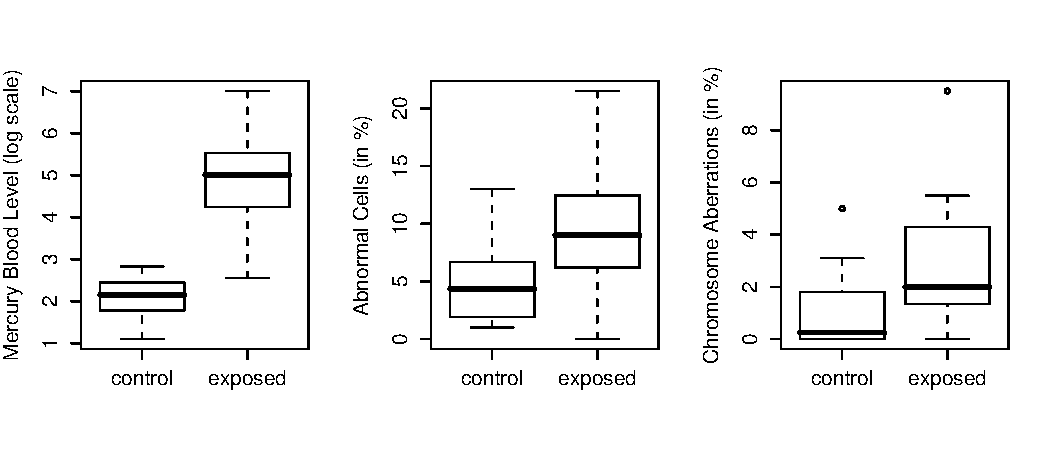
\includegraphics{LegoCondInf-mercuryfish-plot}
\caption{\Robject{mercuryfish} data: 
         Distribution of all three response variables in the exposed group
         and control group. \label{mercurybox}}
\end{center}
\end{figure}

The coherence criterion can be formulated in a simple function
\begin{Schunk}
\begin{Sinput}
R> coherence <- function(data) {
+     x <- t(as.matrix(data))
+     f <- function(y) sum(colSums(x < y) == nrow(x)) - 
+         sum(colSums(x > y) == nrow(x))
+     matrix(apply(x, 2, f), ncol = 1)
+ }
\end{Sinput}
\end{Schunk}
which is now defined as influence function $h$ via the \Rcmd{ytrafo} argument
\begin{Schunk}
\begin{Sinput}
R> poset <- independence_test(mercury + abnormal + ccells ~ 
+     group, data = mercuryfish, ytrafo = coherence, 
+     distribution = exact())
\end{Sinput}
\end{Schunk}
Once the transformations $g$ (a zero-one coding of the exposed and control
group) and $h$ (the coherence criterion) are defined, we enjoy the whole
functionality of the framework, including an exact two-sided $p$-value
\begin{Schunk}
\begin{Sinput}
R> pvalue(poset)
\end{Sinput}
\begin{Soutput}
[1] 4.486087e-06
\end{Soutput}
\end{Schunk}
and density (\Rcmd{dperm}), distribution (\Rcmd{pperm}) and quantile functions 
(\Rcmd{qperm}) of the conditional distribution. When only a small number of
observations is available, it might be interesting to compare the exact
conditional distribution and its approximation via the limiting distribution.
For the \Robject{mercuryfish} data, the relevant parts of 
both distribution functions are shown in Figure~\ref{distplot}. It 
turns out that using the normal approximation would be sufficient for all practical
purposes in this application.

\begin{figure}
\begin{center}
\includegraphics{LegoCondInf-mercuryfish-ppermplot}
\caption{\Robject{mercuryfish} data: 
         Conditional distribution and asymptotic normal approximation 
         for the POSET test. \label{distplot}}
\end{center}
\end{figure}

\section{DISCUSSION}

Conditioning on the observed data is a simple, yet powerful, design
principle for statistical tests. Conceptually, one only needs to choose
an appropriate test statistic and evaluate it for all admissible 
permutations of the data \citep[][gives some examples]{Ernst2004}. 
In practical set ups, an implementation of this
two-step procedure requires a certain amount of programming 
and computing time. Sometimes, permutation tests are even regarded 
as being `computationally impractical'
for larger sample sizes \citep{BalkinMallows2001}. 

The permutation test framework by \cite{StrasserWeber1999} helps us to take
a fresh look at conditional inference procedures and makes at least 
two important contributions: analytic formulae for the 
conditional expectation and covariance and the limiting normal distribution
of a class of multivariate linear statistics. Thus, test statistics can be
defined for appropriately standardized linear statistics and a fast
approximation of the conditional distribution is available, 
especially for large sample sizes. 

It is one mission, if not \textit{the} mission, of statistical computing to
transform new theoretical developments into flexible software tools for the
data analyst. The \Rpackage{coin} package is an attempt to translate 
the theoretical concepts of \cite{StrasserWeber1999} into software tools 
preserving the simplicity and flexibility of 
the theory as closely as possible. With this package, the rather inflexible spanners
currently in use,
such as \Rcmd{wilcox.test} for the Wilcoxon-Mann-Whitney test or
\Rcmd{mantelhaen.test} for the Cochran-Mantel-Haenszel $\chi^2$ test in
\S{} languages and \texttt{NPAR1WAY} for linear rank statistics in \textsf{SAS}
\citep[see the Tables in][for
an overview on procedures implemented in \textsf{StatXact}, \textsf{LogXact},
\textsf{Stata}, \textsf{SAS} and \textsf{Testimate}]{Oster2002,Oster2003}, 
are extended by \Rcmd{independence\_test}, a much more flexible and adjustable spanner.

But who stands to benefit from such a software infrastructure? We argue 
that an improved data analysis is possible in cases when the appropriate 
conditional test is not available from standard software packages.
Statisticians can modify existing test procedures or even try new ideas by
computing directly on the theory. A high-level Lego system is attractive for
both researchers and software developers, because only the transformation $g$ and influence
function $h$ need to be newly implemented, but the burden of implementing a
Monte-Carlo procedure, or even thinking about asymptotics, 
is waived. 

%%Since the \Rpackage{coin} package consists
%%of only a few core functions that need to be tested, the setup of quality
%%assurance tools is rather simple in this case \citep[the need for such tests
%%is obvious,[]{different-:2000}. Many text books
%%\citep[e.g.][]{HollanderWolfe1999} or software manuals \citep[first of all
%%the excellent StatXact handbook by][]{StatXact6} include examples and results
%%of the associated test procedures which have been reproduced with
%%\Rpackage{coin}. 
%%Since the \Rpackage{coin} package is part of the Comprehensive \RR{} Archive
%%Network (CRAN, \url{http://CRAN.R-project.org/}) we have been able to help
%%several people asking `Is the xyz-test available in \RR{}' on the
%%\texttt{r-help} email list with the answer `No, but its only whose 
%%two lines of \RR{} code'. 

With a unifying conceptual framework in mind and a software implementation, such as
\Rpackage{coin}, at hand, we are no longer limited to already published and 
implemented permutation test procedures and are free to define our own transformations and
influence functions, can choose several forms of suitable test statistics and
utilize several methods for the computation or approximation of 
the conditional distribution of the test statistic of interest. Thus, the
construction of an appropriate permutation test, for both classical and
new inference problems, is only a matter of putting together
adequate Lego bricks.

\renewcommand{\baselinestretch}{1}
%%\setlength{\bibsep}{2mm}

\bibliographystyle{plainnat}
\bibliography{LegoCondInf}

\clearpage

\setkeys{Gin}{width=0.9\textheight}
\pagestyle{empty}

\end{document}
